\chapter{Latent Space and Domain Embedding t-SNE Filtered by User}

We plotted the latent space and domain embedding t-SNEs with the DDPG agent trained on the MTF transform and one-hot encoding for both the model initially trained and the model that was trained with extended epochs and agent steps.
We felt that no additional conclusions could be drawn from these plots and as such did not include them in our main discussion section but include them here for posterity.

\begin{figure}[b]
	\centering
	\begin{subfigure}{0.3\textwidth}
		\centering
		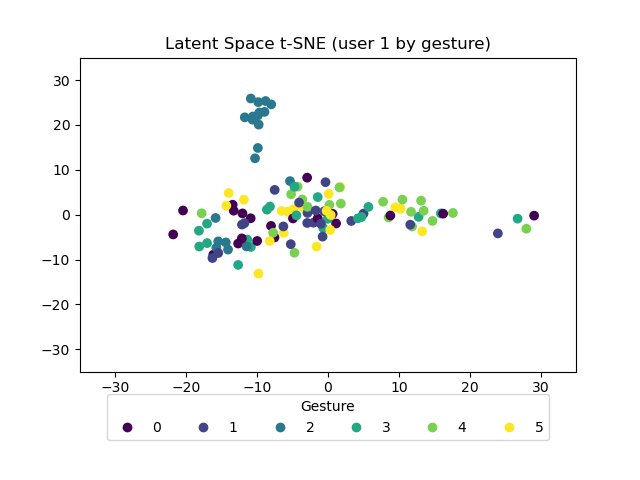
\includegraphics[width=\textwidth]{figures/short/short_ls_u1}
		\caption{t-SNE by gesture for User 1}
	\end{subfigure}
	\hfill
	\begin{subfigure}{0.3\textwidth}
		\centering
		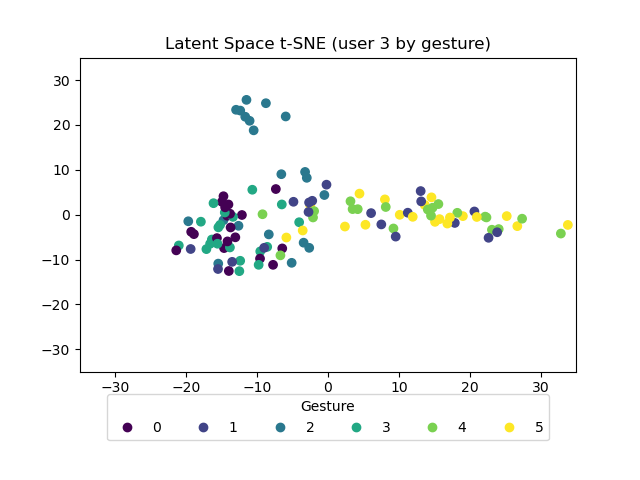
\includegraphics[width=\textwidth]{figures/short/short_ls_u3}
		\caption{t-SNE by gesture for User 3}
	\end{subfigure}
	\hfill
	\begin{subfigure}{0.3\textwidth}
		\centering
		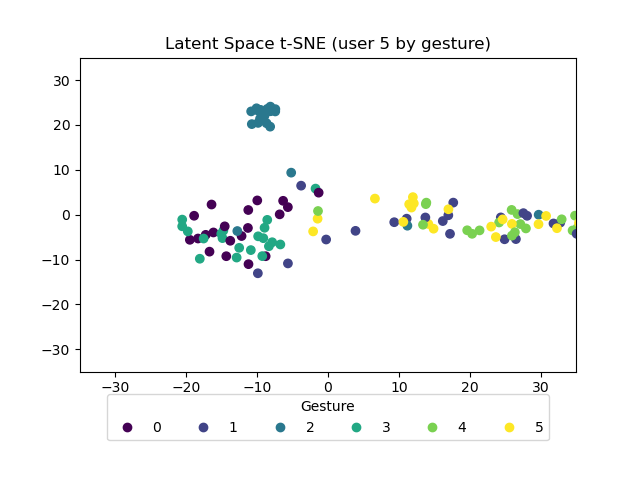
\includegraphics[width=\textwidth]{figures/short/short_ls_u5}
		\caption{t-SNE by gesture for User 5}
	\end{subfigure}
	\hfill
	\begin{subfigure}{0.3\textwidth}
		\centering
		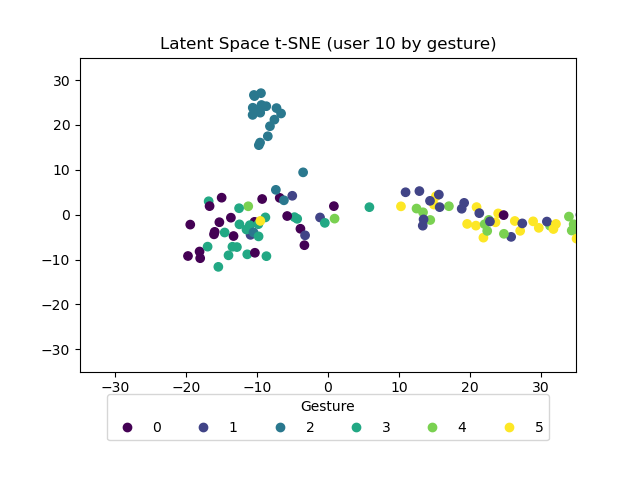
\includegraphics[width=\textwidth]{figures/short/short_ls_u10}
		\caption{t-SNE by gesture for User 10}
	\end{subfigure}
	\hfill
	\begin{subfigure}{0.3\textwidth}
		\centering
		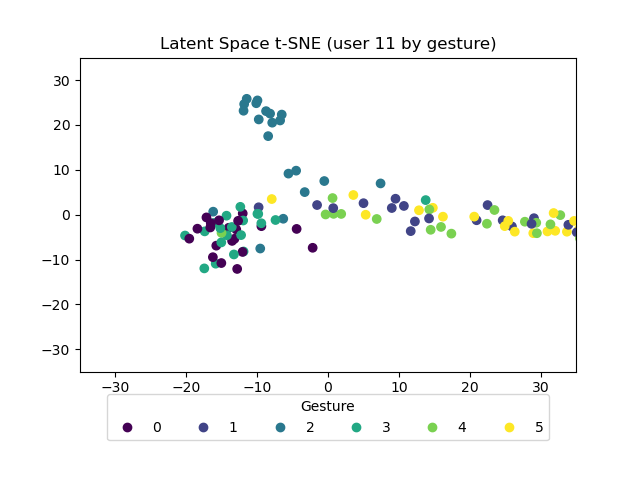
\includegraphics[width=\textwidth]{figures/short/short_ls_u11}
		\caption{t-SNE by gesture for User 11}
	\end{subfigure}
	\hfill
	\begin{subfigure}{0.3\textwidth}
		\centering
		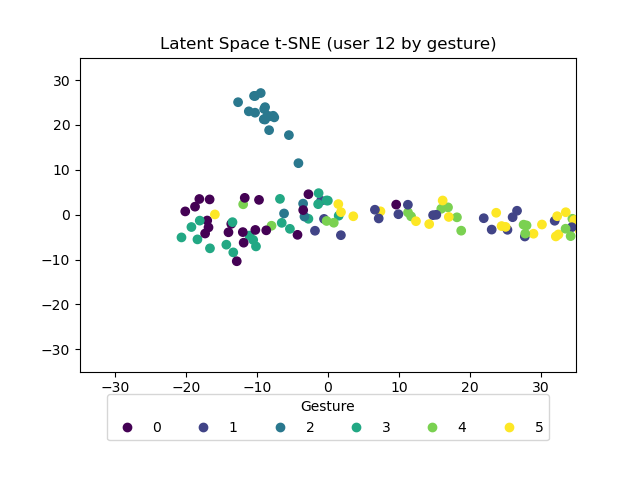
\includegraphics[width=\textwidth]{figures/short/short_ls_u12}
		\caption{t-SNE by gesture for User 12}
	\end{subfigure}
	\hfill
	\begin{subfigure}{0.3\textwidth}
		\centering
		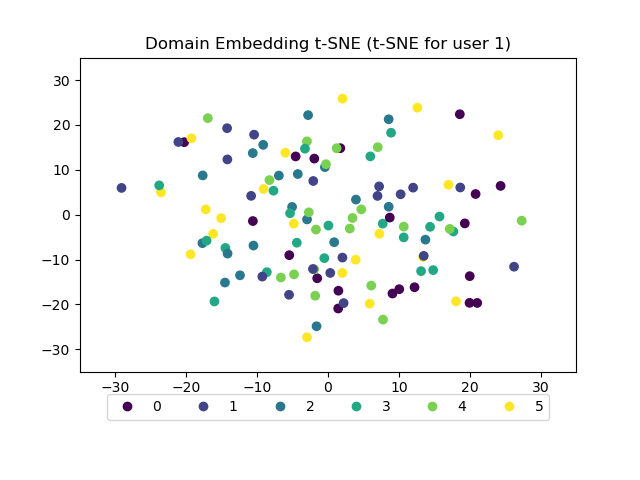
\includegraphics[width=\textwidth]{figures/short/short_de_u1}
		\caption{t-SNE by gesture for User 1}
	\end{subfigure}
	\hfill
	\begin{subfigure}{0.3\textwidth}
		\centering
		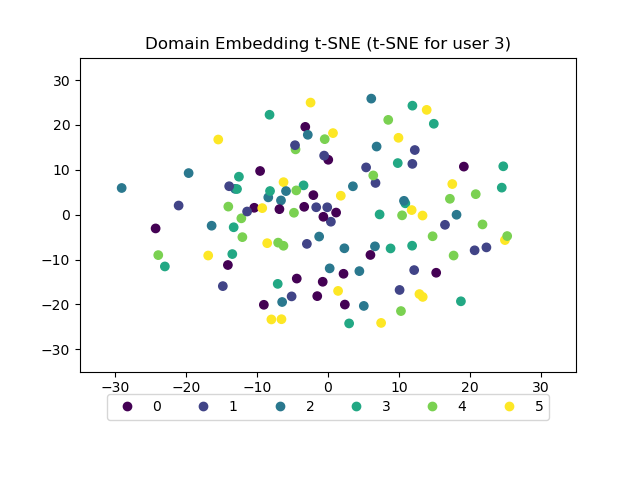
\includegraphics[width=\textwidth]{figures/short/short_de_u3}
		\caption{t-SNE by gesture for User 3}
	\end{subfigure}
	\hfill
	\begin{subfigure}{0.3\textwidth}
		\centering
		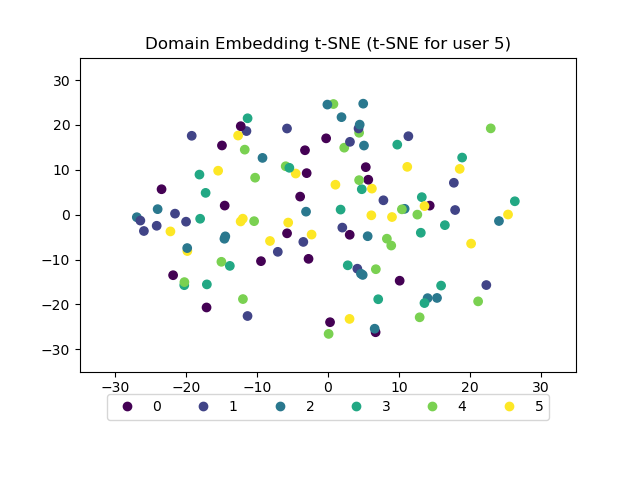
\includegraphics[width=\textwidth]{figures/short/short_de_u5}
		\caption{t-SNE by gesture for User 5}
	\end{subfigure}
	\hfill
	\begin{subfigure}{0.3\textwidth}
		\centering
		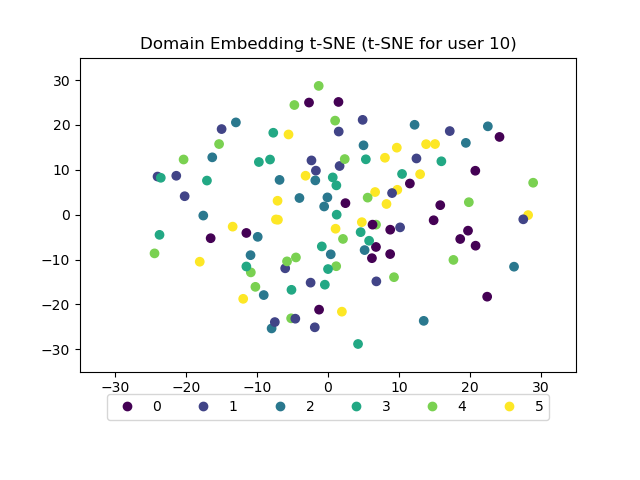
\includegraphics[width=\textwidth]{figures/short/short_de_u10}
		\caption{t-SNE by gesture for User 10}
	\end{subfigure}
	\hfill
	\begin{subfigure}{0.3\textwidth}
		\centering
		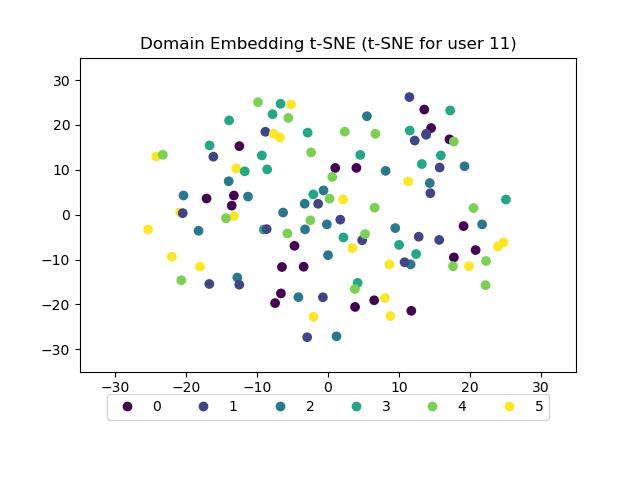
\includegraphics[width=\textwidth]{figures/short/short_de_u11}
		\caption{t-SNE by gesture for User 11}
	\end{subfigure}
	\hfill
	\begin{subfigure}{0.3\textwidth}
		\centering
		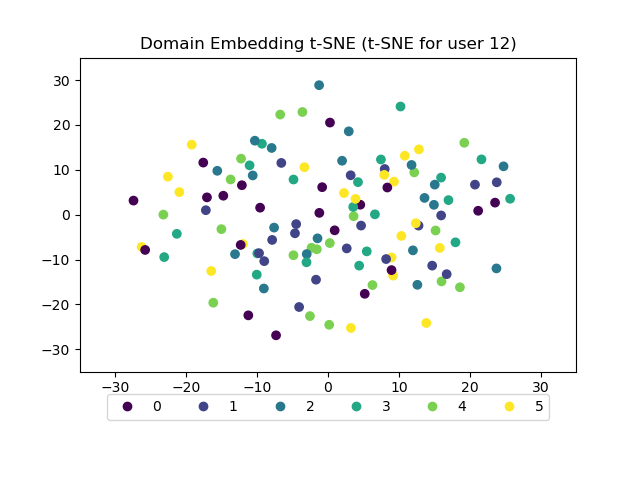
\includegraphics[width=\textwidth]{figures/short/short_de_u12}
		\caption{t-SNE by gesture for User 12}
	\end{subfigure}
	\hfill
	\caption{t-SNEs of the latent space and domain embeddings produced by PPO with one-hot encoding and MTF transformation with the initial training time, filtered by User.}
\end{figure}

\begin{figure}[b]
	\centering
	\begin{subfigure}{0.3\textwidth}
		\centering
		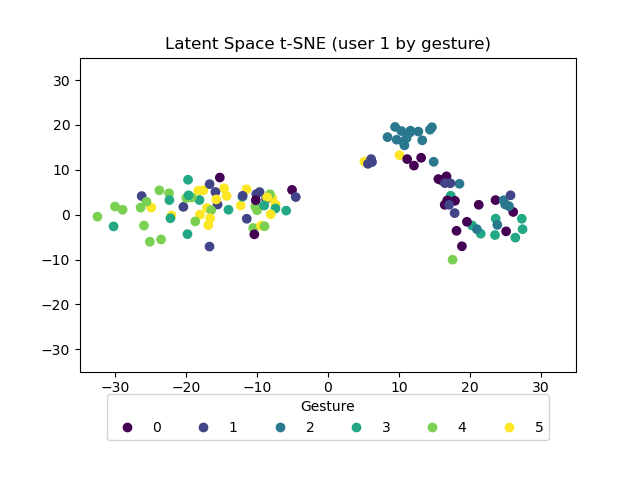
\includegraphics[width=\textwidth]{figures/extended/long_ls_u1}
		\caption{t-SNE by gesture for User 1}
	\end{subfigure}
	\hfill
	\begin{subfigure}{0.3\textwidth}
		\centering
		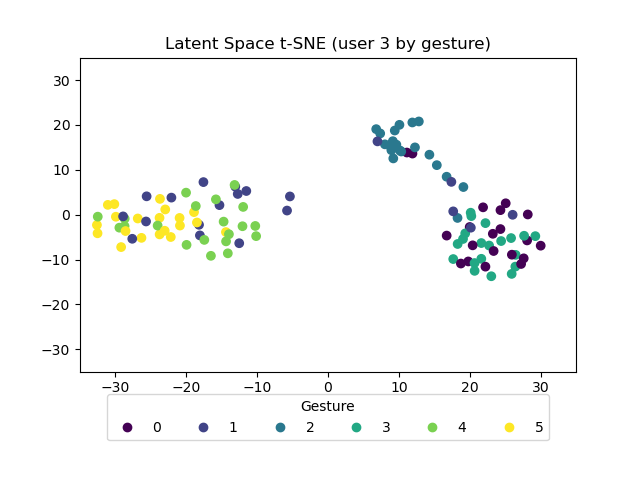
\includegraphics[width=\textwidth]{figures/extended/long_ls_u3}
		\caption{t-SNE by gesture for User 3}
	\end{subfigure}
	\hfill
	\begin{subfigure}{0.3\textwidth}
		\centering
		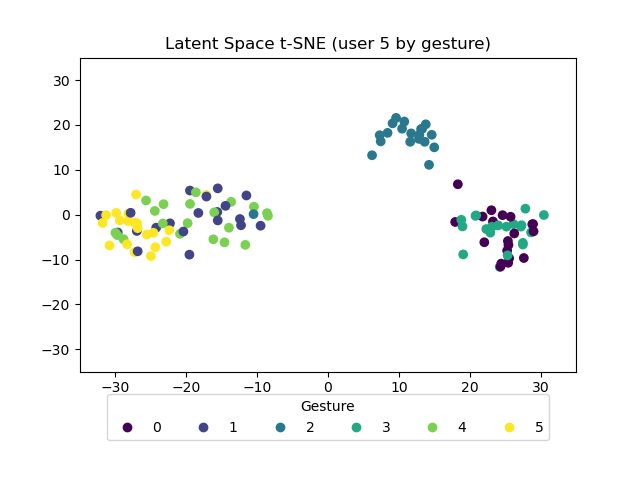
\includegraphics[width=\textwidth]{figures/extended/long_ls_u5}
		\caption{t-SNE by gesture for User 5}
	\end{subfigure}
	\hfill
	\begin{subfigure}{0.3\textwidth}
		\centering
		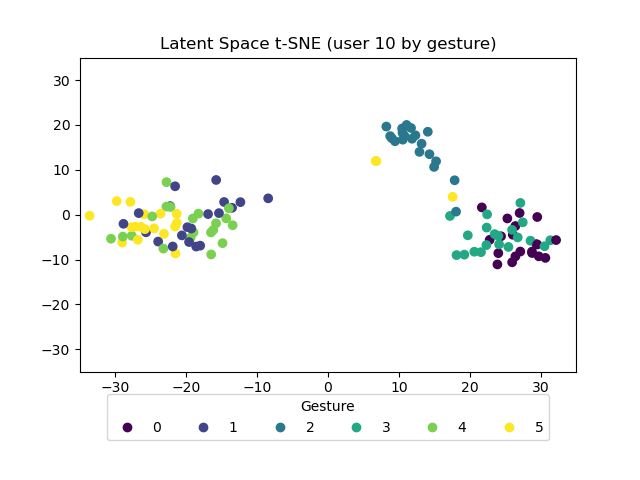
\includegraphics[width=\textwidth]{figures/extended/long_ls_u10}
		\caption{t-SNE by gesture for User 10}
	\end{subfigure}
	\hfill
	\begin{subfigure}{0.3\textwidth}
		\centering
		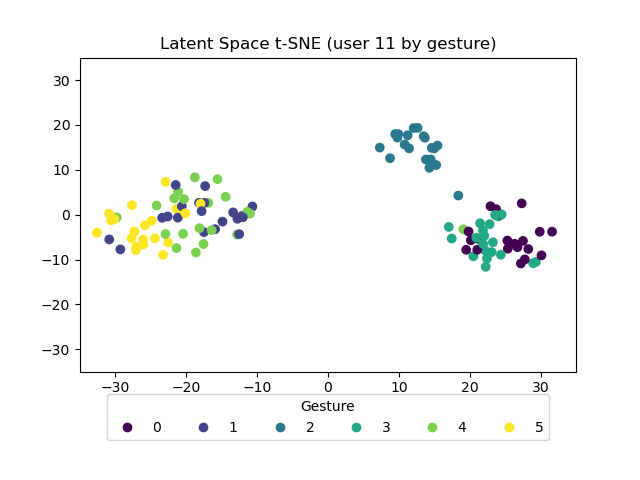
\includegraphics[width=\textwidth]{figures/extended/long_ls_u11}
		\caption{t-SNE by gesture for User 11}
	\end{subfigure}
	\hfill
	\begin{subfigure}{0.3\textwidth}
		\centering
		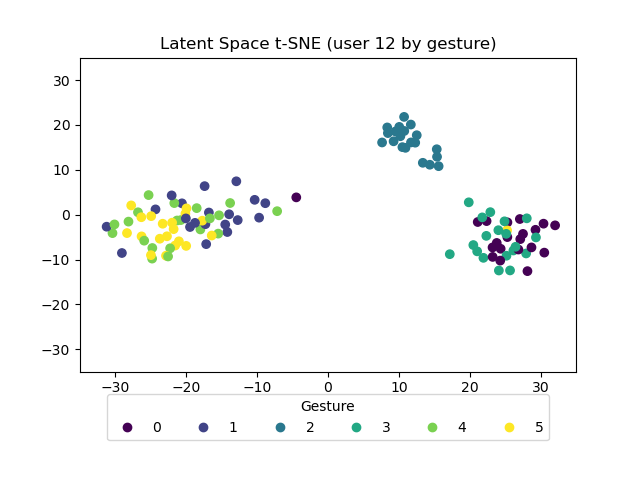
\includegraphics[width=\textwidth]{figures/extended/long_ls_u12}
		\caption{t-SNE by gesture for User 12}
	\end{subfigure}
	\hfill
	\begin{subfigure}{0.3\textwidth}
		\centering
		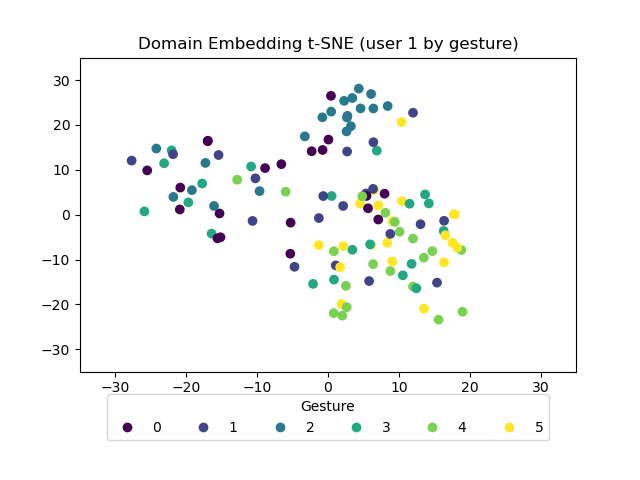
\includegraphics[width=\textwidth]{figures/extended/long_de_u1}
		\caption{t-SNE by gesture for User 1}
	\end{subfigure}
	\hfill
	\begin{subfigure}{0.3\textwidth}
		\centering
		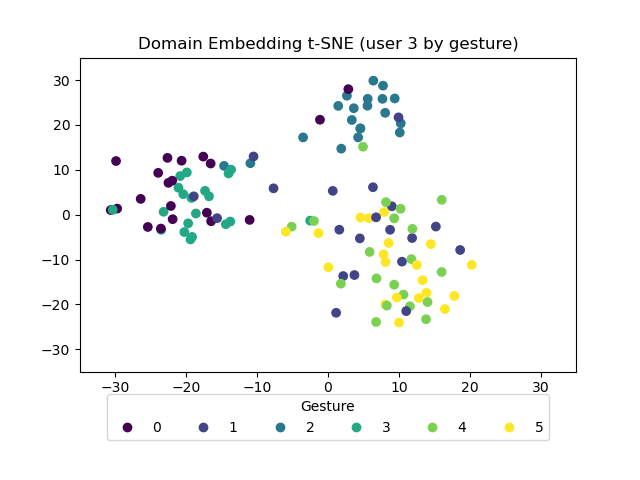
\includegraphics[width=\textwidth]{figures/extended/long_de_u3}
		\caption{t-SNE by gesture for User 3}
	\end{subfigure}
	\hfill
	\begin{subfigure}{0.3\textwidth}
		\centering
		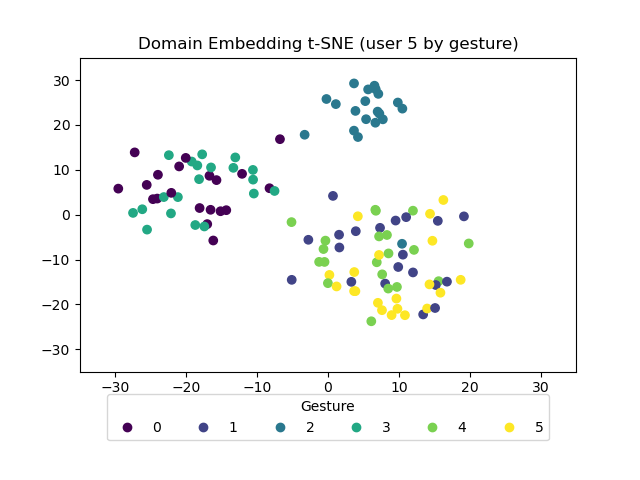
\includegraphics[width=\textwidth]{figures/extended/long_de_u5}
		\caption{t-SNE by gesture for User 5}
	\end{subfigure}
	\hfill
	\begin{subfigure}{0.3\textwidth}
		\centering
		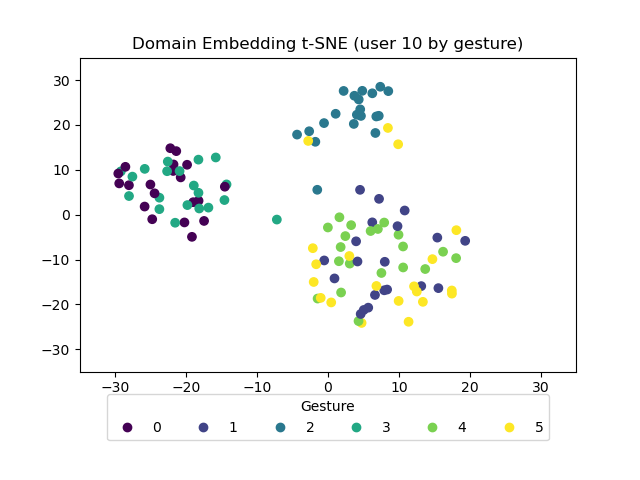
\includegraphics[width=\textwidth]{figures/extended/long_de_u10}
		\caption{t-SNE by gesture for User 10}
	\end{subfigure}
	\hfill
	\begin{subfigure}{0.3\textwidth}
		\centering
		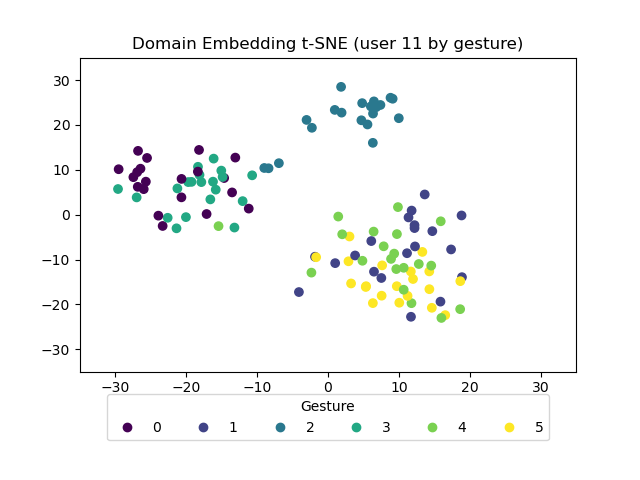
\includegraphics[width=\textwidth]{figures/extended/long_de_u11}
		\caption{t-SNE by gesture for User 11}
	\end{subfigure}
	\hfill
	\begin{subfigure}{0.3\textwidth}
		\centering
		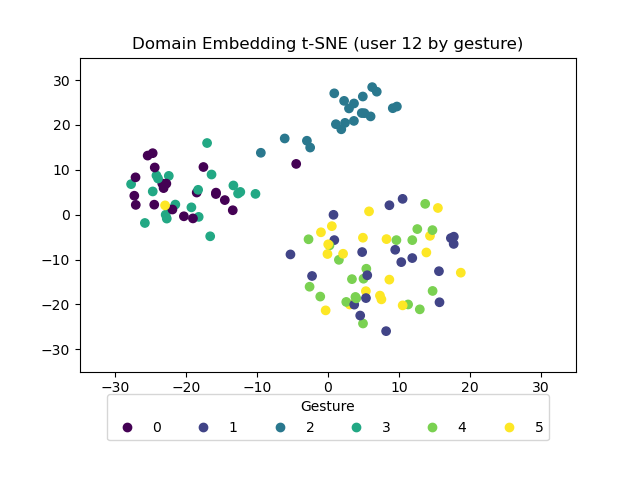
\includegraphics[width=\textwidth]{figures/extended/long_de_u12}
		\caption{t-SNE by gesture for User 12}
	\end{subfigure}
	\hfill
	\caption{t-SNEs of the latent space and domain embeddings produced by PPO with one-hot encoding and MTF transformation with extended training time, filtered by User.}
\end{figure}